\documentclass{article}
\usepackage{hyperref}
\usepackage{lipsum}
\usepackage{mathtools}
\usepackage[margin=1in,includefoot]{geometry}
\usepackage{fancyhdr}
\pagestyle{fancy}
\usepackage{amsmath}
%\usepackage{amslatex}
\fancyhead{}
%\fancyfoot{}
%\fancyfoot[R]{\thepage\}
\begin{document}

%\usepackage{fancyhdr}
%\pagestyle{fancy}
%\fancyhead{}
%\fancyfoot{}
%\fancyfoot[R]{\thepage\}


\begin{titlepage}

   \begin{center}

   \line(1,0){300}\\
   [0.25in]
   \huge\bfseries CMPT 419: Assigment 1 Fall 2018\\
   [2mm]
   \line(1,0){200}\\
   [1.5cm]
   \textsc{Echo Liu}\\
   [0.75cm]
   \textsc{Linear Regression}\\
   \end{center}

\end{titlepage}

\section{Question 1}\label{sec:question1}

\begin{enumerate}
    % part 1
    \item The nature of this distribution is of a multionomial distribution,
    \\ as such its parameters are as follows
    \\ $f(x_{1},...,x_{k};n,p_{1},...,p_{k})= Pr(X_{1}=x_{1} \hspace{0.1cm} and ... and \hspace{0.1cm} X_{k}=x_{k})=\frac{n!}{x_{1}!...x_{k}!}*p_{1}\times...\times p_{k}$
    \\ where each $p_{k}$ can be thought of as $\mu_{k}$ and $\sum_{n=1}^{k} x_{i} = n$
    
    % part 2
    \item Values of each $\mu_{i} $ is $\frac{1}{3}$

    % part 3
    \item Let $\Omega$  be our sample space, let $ B$ be our event space and 
    \\ $P$ be our probability function and j be an index that denotes
    \\ that party j is elected, then:
    \\ $\Omega$ : \[\left\{[0,0,1],[1,0,0],[0,1,0]\right\}\] where we compute
    \\ the permutations of [[0,0,1],[1,0,0],[0,1,0]], [[1,0,0],[0,1,0],[0,0,1]]

     \par $B$: \[\left\{0,1,2\right\}\] 
     in otherwords each element in this set is an index
     set into set $\Omega$ where each index denotes that a particular party
     is elected for example if I computed $\Omega_{b}$ where b is in set $B$ 
     then I am essentially indexing the bth element of Omega e.g
     $\Omega_{1}$=[1,0,0] then in index j, we get our outcome if and only if
     j=b i.e if j=b, then P evaluates to 1, 0 otherwise, where j is an index
     into the bth element
     In otherwords
     \[ P(j) = 
        \begin{cases}
        	1 & \text{if b=j}\\
        	0 & \text{otherwise}
        \end{cases}
      
     \]
     
     %part 4
     \item For this question, imagine oneself as an auditor, auditing election practices. As such if a politician wanted to rig the election they'd hire a partison auditor. As such the components of the alpha
     \\vector would have components [\alpha_{1},\alpha_{2},...,\alpha_{i}] where for party k, we use a one hot encoding scheme and
     \\ subsitute in our Dirshlet Distribution as appropiate.

     %part 5
     \item We assume that when a given party is elected, that this distribution takes on a Dirchlet distribution.
     \\ Moreover, we take all the alpha parameters and set them to 1. In otherwords we are encoding an uniform
     \\ Dirshlet prior, with a one hot encoding scheme about the alpha vector for the Green party.

     %part 6
     \item Assuming each party has equal probability of winning, we take the Dirschlet distribution and intergrate as appropiate.

%\section{Question 2}\label{sec:question2}


     


\end{enumerate}

\pagebreak

\section{Question 2}\label{sec:questiontwo}

Basic idea: Assign a subscript i, to each beta to form \beta_{i}
\\
Hence\hspace{0.5cm} we\hspace{0.5cm} do\hspace{0.5cm} the\hspace{0.5cm} following \hspace{0.5cm}
\\

\begin{math}

$p( \vec{t}|\vec{w}^{T}\phi( \vec{x_{n}} ),\beta_{n}^{-1} )$
$=\prod_{n=1}^{N} \frac{\sqrt{\beta_{n}}}{\sqrt{2\pi}} exp((-\frac{\beta_{n}}{2} (t_{n}-\vec{w}^{T}\phi(\vec{x_{n}})) ))$

\end{math}
\\
Then \hspace{0.5cm} we \hspace{0.5cm} change  \hspace{0.5cm} the \hspace{0.5cm} product \hspace{0.5cm}
\\
to\hspace{0.5cm}a\hspace{0.5cm}summation\hspace{0.5cm}

$=\sum_{n=1}^{N} ln(\frac{\sqrt{\beta_{n}}}{\sqrt{2\pi}} exp((-\frac{\beta_{n}}{2} (t_{n}-\vec{w}^{T}\phi(\vec{x_{n}})) )))

\\
We\hspace{0.5cm}approach\hspace{0.5cm}each\hspace{0.5cm}variable\hspace{0.5cm}as\hspace{0.5cm}a\hspace{0.5cm}joint
\\
density\hspace{0.5cm}function\hspace{0.5cm}so\hspace{0.5cm}we\hspace{0.5cm}obtain\hspace{0.5cm}the\hspace{0.5cm}following:
\\

$=\sum_{n=1}^{N}ln(2\pi)^{-\frac{1}{2}} + \sum_{n=1}^{N} ln(\beta_{n}^{-\frac{1}{2}}) + \sum_{n=1}^{N}((\frac{1}{2}\beta_{n}(t_{n}-\vec{w}^{T}\phi(\vec{x_{n}}))) $

\\
One\hspace{0.5cm}can\hspace{0.5cm}then\hspace{0.5cm}simplify\hspace{0.5cm}the\hspace{0.5cm}expression\hspace{0.5cm}further
\\
by\hspace{0.5cm}moving\hspace{0.5cm}the\hspace{0.5cm}1/2\hspace{0.5cm}to\hspace{0.5cm}the\hspace{0.5cm}front

Our \hspace{0.5cm}sum \hspace{0.5cm}of \hspace{0.5cm}squares \hspace{0.5cm}error \hspace{0.5cm}term \hspace{0.5cm}is \hspace{0.5cm}the \hspace{0.5cm}third\hspace{0.5cm} term
\\

\pagebreak

\section{Question 3}\label{sec:questionthree}

\item Part\hspace{0.5cm} 1: \hspace{0.5cm}The\hspace{0.5cm} answer \hspace{0.5cm}is \hspace{0.5cm}no\hspace{0.5cm}:\hspace{0.5cm} the \hspace{0.5cm}reason \hspace{0.5cm}being \hspace{0.5cm}is \hspace{0.5cm}that\hspace{0.5cm} the \hspace{0.5cm}validation\hspace{0.5cm} set\hspace{0.5cm} could\hspace{0.5cm} possibly\hspace{0.5cm} 
provide \hspace{0.5cm}the\hspace{0.5cm} model\hspace{0.5cm} with\hspace{0.5cm} some\hspace{0.5cm} insights\hspace{0.5cm} into\hspace{0.5cm} the\hspace{0.5cm} actual\hspace{0.5cm} model\hspace{0.5cm}

\\

\item The\hspace{0.5cm} answer\hspace{0.5cm} is \hspace{0.5cm}no\hspace{0.5cm},\hspace{0.5cm} your\hspace{0.5cm} data\hspace{0.5cm} could\hspace{0.5cm} happen\hspace{0.5cm} to\hspace{0.5cm} be\hspace{0.5cm} modeled\hspace{0.5cm} as\hspace{0.5cm} a\hspace{0.5cm} straight\hspace{0.5cm} line\hspace{0.5cm} and\hspace{0.5cm} thus\hspace{0.5cm} increasing\hspace{0.5cm} the\hspace{0.5cm} polynomial \hspace{0.5cm}degree\hspace{0.5cm}will\hspace{0.5cm}increase\hspace{0.5cm}the\hspace{0.5cm}training\hspace{0.5cm}error

\item \hspace{0.5cm}The\hspace{0.5cm} answer\hspace{0.5cm} is\hspace{0.5cm} yes\hspace{0.5cm}:\hspace{0.5cm}
\hspace{0.5cm}by\hspace{0.5cm}definition\hspace{0.5cm}regularizion\hspace{0.5cm}penalizes\hspace{0.5cm}model
\hspace{0.5cm}complexity

\pagebreak

\section{Question 4}\label{sec:questionfour}


%\hspace{0.1cm}We\hspace{0.1cm}are\hspace{0.1cm}essentially\hspace{0.5cm}trying\hspace{0.5cm}
%to\hspace{0.5cm}find\hspace{0.5cm}the\hspace{0.5cm}gradient\hspace{0.5cm}of\hspace{0.5cm}5
%the\hspace{0.5cm}elastic\hspace{0.5cm}net\hspace{0.5cm}regression\hspace{0.5cm}function\hspace{0.5cm}
We are essentially trying to find the gradient of the elastic net regression function

\\ Thus our error function goes as follows
\\$E_{D}(\vec{w})=\frac{1}{2}\sum_{n=1}^{N} \DeclarPairedDelimeter\set\{t_{n}-\vec{w^{T}}\phi(\vec{x_{n}})\}+ \sum_{i=1}^{J_{1}} \lambda_{i}|w_{i}|+ \sum_{j=1}^{J_{2}} \frac{\lambda_{j}}{2}w_{j}^{2}$
\\ Therefore our gradient goes as follows, our approach is that we use the matrix form of the quadratic
\\ i.e think of $x^{2}$ and $\vec{x}^{T}\vec{x}$ as logically equivalent, thus we obtain the following for the gradient 
\\$\nabla E_{D}(\vec{w})=-\sum_{n=1}^{N}\DeclaredPairedDelimeter\set\{t_{n}-\vec{w}^{T}\phi(\vec{x}_{n})\}\vec{\phi}^{T}(\vec{x}_{n})+\frac{1}{2}\sum_{i=1}^{J_{1}}\lambda_{i}\frac{\vec{w}}{|w_{i}|}+\sum_{j=1}^{J_{2}}\lambda_{j}|w_{j}|$


\pagebreak

\section{Question 5}\label{sec:Question5}

\begin{enumerate}
	\item Responses to section section "Getting Started"
	\\ The country that had the highest child mortality rate in 1990 is Libera
	\\ with value of 160.8
	\\ The country that had the highest child mortality rate in 2011 is Sierra Leone
	\\ with value 119.2
	\\ The API handles the NaN values by filling them with random entries, in practice
	\\ this might not be the correct thing to do.

	\item Response to section "Polynomial Regression"
	\\
	\begin{figure}[h!]
		\centering
		\begin{subfigure}[b]{0.4\linewidth}
			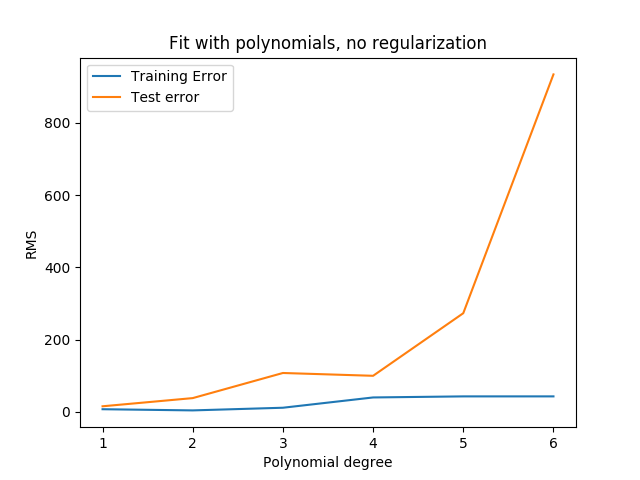
\includegraphics[width=\linewidth]{Error_vs_PolyDegree.png}
			\caption{Non normalized features, we plot the error in RMS versus polynomial degree as one can see the testing error is greater than training error}
		\end{subfigure}
		
	\end{figure}
\end{enumerate}

\pagebreak



\section{Question 5 Continued}\label{sec:Question5Continued}

\begin{enumerate}
	\begin{figure}[h!]
		\centering
		\begin{subfigure}[b]{0.4\linewidth}
			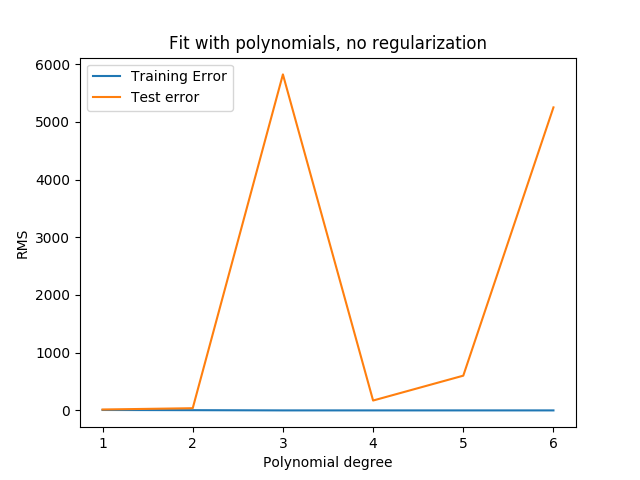
\includegraphics[width=\linewidth]{Error_vs_PolyDegreenorm.png}
			\caption{We run our program again, normalizing our features}
		\end{subfigure}
	\end{figure}

\end{enumerate}

\pagebreak

\section{Question 5 Continued}\label{sec:Question5Continued}
\begin{enumerate}
	\begin{figure}[h!]
		\centering
		\begin{subfigure}[b]{0.4\linewidth}
			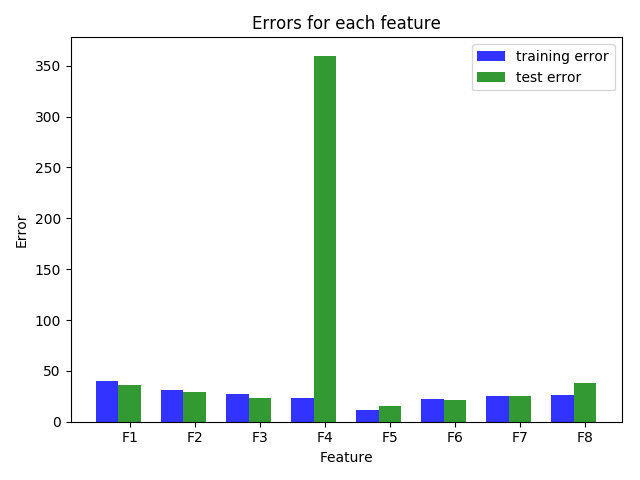
\includegraphics[width=\linewidth]{Bargraph.png}
			\caption{As one can see, there is a spike in error in one of our features, suggesting a polynomial fit might not best describe out data}
		\end{subfigure}
	\end{figure}
\end{enumerate}
 

\pagebreak

\section{Question 5 Continued}\label{sec:Question5Continued}

\begin{enumerate}
	\begin{figure}[h!]
		\centering
		\begin{subfigure}[b]{0.4\linewidth}
			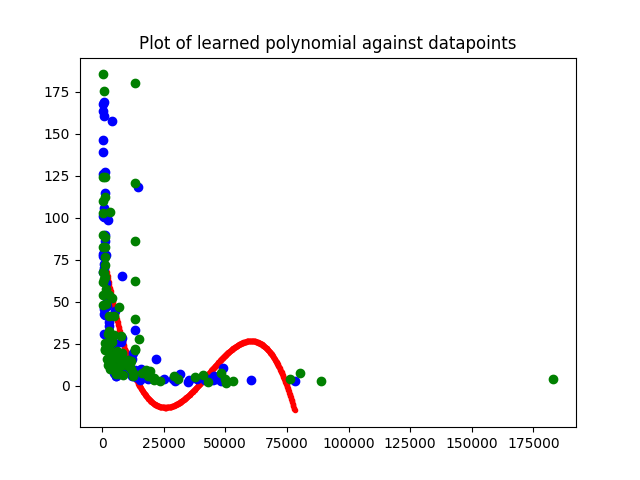
\includegraphics[width=\linewidth]{GNICurve.png}
			\caption{Our curve fitted against our training and test points with our GNI feature, as one can see the polynomial does not best fit our data}
		\end{subfigure}
		
	\end{figure}
\end{enumerate}


\pagebreak

\section{Question 5 Continued}\label{sec:Question5Continued}

\begin{figure}[h!]
	\centering
	\begin{subfigure}[b]{0.4\linewidth}
		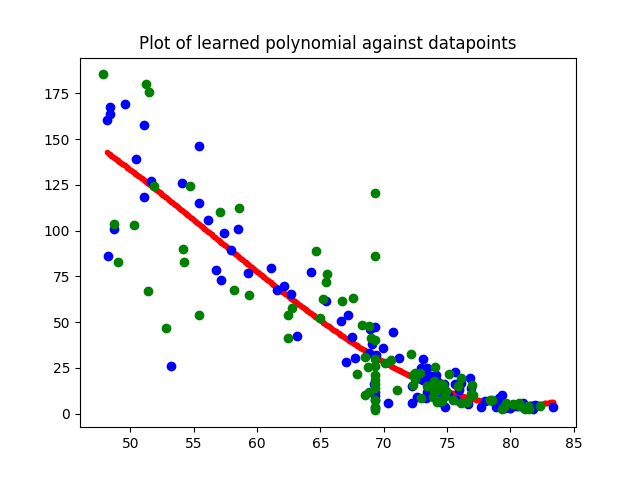
\includegraphics[width=\linewidth]{LifeExpectancy.png}
		\caption{Our curve fitted against our training and test points with our Life Expectancy feature,as one can see the data isn't best represented by a polynomial of degree 3}
	\end{subfigure}
\end{figure}

\pagebreak

\section{Question 5 Continued}\label{sec:Question5Continued}

\begin{figure}[h!}
	\centering
	\begin{subfigure}[b]{0.4\linewidth}
		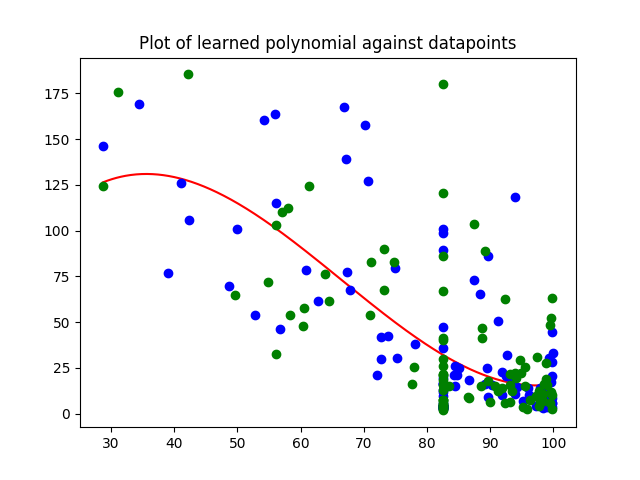
\includegraphics[width=\linewidth]{Literacypolynomial.png}
		\caption{Our curve fitted against our training and test points with our Literacy Expectancy feature, as one can see a deg 3 polynomial does not best fit our data}
	\end{subfigure}
\end{figure}

\pagebreak
\section{Question 5 Continued}\label{sec:Question5Continued}

\\
Response to section "ReLU Basis Function"

\begin{figure}[h!]
	\centering
	\begin{subfigure}[b]{0.4\linewidth}
		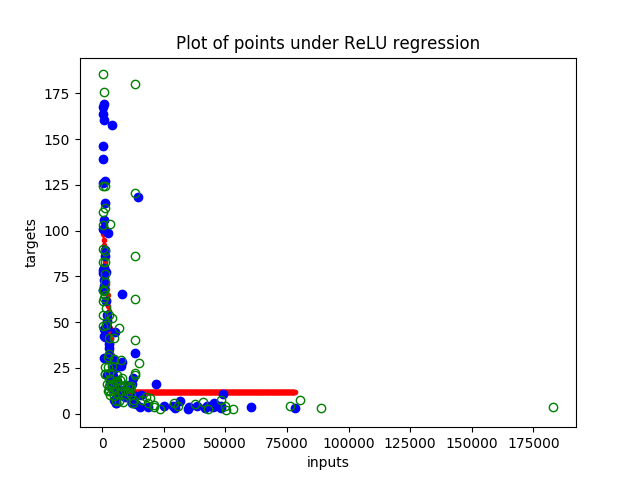
\includegraphics[width=\linewidth]{ReLu.png}
		\caption{Our curve fitted against our data [test and training] points, with training and testing error resp being 20.59 and 24.199}
	\end{subfigure}
\end{figure}

\pagebreak
\section {Question 5 End} \label{sec:Question5End}

\\
Response to section "Polynomial Regression, Regularization"

\begin{figure}[h!]
	\centering
	\begin{subfigure}[b]{0.4\linewidth}
		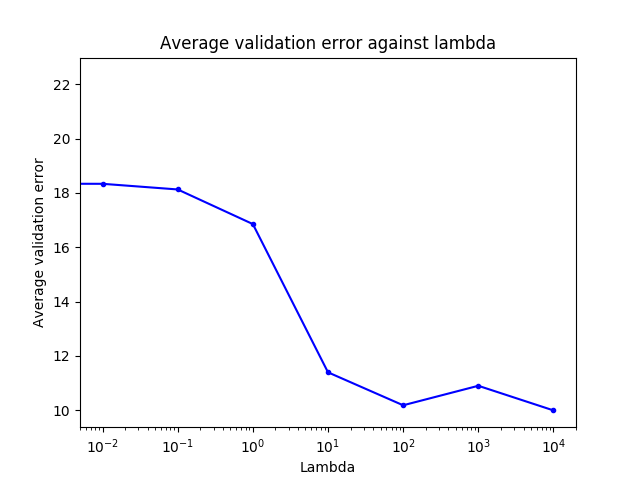
\includegraphics[width=\linewidth]{VL.png}
		\caption{As one can see in the following diagram, the best value for lambda is 100 or ten squared and tied with 10000 or 10 to the four}
	\end{subfigure}
\end{figure}


\end{document}
